% interactcadsample.tex
% v1.03 - April 2017

\documentclass[]{interact}

\usepackage{epstopdf}% To incorporate .eps illustrations using PDFLaTeX, etc.
\usepackage{subfigure}% Support for small, `sub' figures and tables
%\usepackage[nolists,tablesfirst]{endfloat}% To `separate' figures and tables from text if required

\usepackage{natbib}% Citation support using natbib.sty
\bibpunct[, ]{(}{)}{;}{a}{}{,}% Citation support using natbib.sty
\renewcommand\bibfont{\fontsize{10}{12}\selectfont}% Bibliography support using natbib.sty

\theoremstyle{plain}% Theorem-like structures provided by amsthm.sty
\newtheorem{theorem}{Theorem}[section]
\newtheorem{lemma}[theorem]{Lemma}
\newtheorem{corollary}[theorem]{Corollary}
\newtheorem{proposition}[theorem]{Proposition}

\theoremstyle{definition}
\newtheorem{definition}[theorem]{Definition}
\newtheorem{example}[theorem]{Example}

\theoremstyle{remark}
\newtheorem{remark}{Remark}
\newtheorem{notation}{Notation}


% tightlist command for lists without linebreak
\providecommand{\tightlist}{%
  \setlength{\itemsep}{0pt}\setlength{\parskip}{0pt}}



\usepackage{lscape}
\usepackage{hyperref}
\usepackage[utf8]{inputenc}
\def\tightlist{}
\usepackage{xcolor}
\definecolor{orange-red}{rgb}{1.0, 0.27, 0.0}
\newcommand{\svp}[1]{{\textcolor{orange-red}{#1}}}
\newcommand*{\Perm}[2]{{}^{#1}\!P_{#2}}%

\usepackage{booktabs}
\usepackage{longtable}
\usepackage{array}
\usepackage{multirow}
\usepackage{wrapfig}
\usepackage{float}
\usepackage{colortbl}
\usepackage{pdflscape}
\usepackage{tabu}
\usepackage{threeparttable}
\usepackage{threeparttablex}
\usepackage[normalem]{ulem}
\usepackage{makecell}
\usepackage{xcolor}

\begin{document}


\articletype{ARTICLE TEMPLATE}

\title{Why is it that statistical tests for residuals are not widely
used? An explanation using visual inference.}


\author{\name{Weihao Li$^{a}$, Dianne Cook$^{a}$, Emi
Tanaka$^{a}$, Susan VanderPlas$^{b}$}
\affil{$^{a}$Department of Econometrics and Business Statistics, Monash
University, Clayton, VIC, Australia; $^{b}$Department of Statistics,
University of Nebraska, Lincoln, Nebraska, USA}
}

\thanks{CONTACT Weihao
Li. Email: \href{mailto:weihao.li@monash.edu}{\nolinkurl{weihao.li@monash.edu}}, Dianne
Cook. Email: \href{mailto:dicook@monash.edu}{\nolinkurl{dicook@monash.edu}}, Emi
Tanaka. Email: \href{mailto:emi.tanaka@monash.edu}{\nolinkurl{emi.tanaka@monash.edu}}, Susan
VanderPlas. Email: \href{mailto:susan.vanderplas@unl.edu}{\nolinkurl{susan.vanderplas@unl.edu}}}

\maketitle

\begin{abstract}
Abstract to fill.
\end{abstract}

\begin{keywords}
data visualization; visual inference; hypothesis testing; residual
plots;
\end{keywords}

Title (jokes: finding the pattern in residual tests) (why using
visulization is important in regression diagnostics? an explanation
using visual inference) (a picture is worth a thousand word) (a plot is
worth a thousand test: )

(title refine - rank: low)

(fix the tense issue - rank: low)

(fix the notation issue (bold?) - rank: low)

\hypertarget{introduction}{%
\section{Introduction}\label{introduction}}

(introduction refine - rank: low)

\begin{quote}
\emph{``Since all models are wrong the scientist must be alert to what
is importantly wrong.''} \citep{box1976science}
\end{quote}

Diagnostics are the key to determining whether there is anything
importantly wrong with a model. In linear regression analysis, residuals
from the model fit are commonly used. Residuals summarise what is not
captured by the model, and thus provide the capacity to identify what
might be wrong.

We can assess residuals in multiple ways. Residuals might be plotted, as
a histogram or quantile-quantile plot to examine the distribution. Using
the classical normal linear regression model as an example, if the
distribution is symmetric and unimodal, we consider it well-behaved. But
if the distribution is skewed, bimodal, multimodal, or contains
outliers, there is cause for concern. One could also inspect the
distribution by conducting a goodness of fit test, such as the
Shapiro-Wilk Normality test \citep{shapiro1965analysis}.

More typically, residuals will be plotted, as a scatter plot against the
predicted values and each of the explanatory variables to scrutinize
their relationships. If there are any visually discoverable patterns,
the model is potentially misspecified. In general, one looks for
noticeable departures from the model like non-linear dependency or
heteroskedasticity. However, correctly judging a residual plot where no
pattern exists is a painstakingly difficult task for humans (?citation).
It is especially common, particularly among new data analysts, to report
patterns when an experienced one might quickly conclude that there are
none. It is also possible to conduct hypothesis tests for non-linear
dependence \citep{ramsey_tests_1969}, and use a Breusch-Pagan test
\citep{breusch_simple_1979} for heteroskedasticity.

Abundance of literature describe appropriate diagnostic methods for
linear regression: \citet{draper1998applied},
\citet{montgomery1982introduction}, \citet{belsley_regression_1980},
\citet{cook_applied_1999} and \citet{cook1982residuals}. All of these
writings consider plotting of residuals to be a standard technique that
should be examined routinely in all regression modelling problems. In
addition, \citet{draper1998applied} and \citet{belsley_regression_1980}
believe that residual plots are usually very revealing when the
assumptions are violated. \citet{cook_applied_1999} thinks formal tests
and graphical procedures are complementary and both have a place in
residual analysis, but they focus on graphical methods rather than on
formal testing, as they are easier to use.
\citet{montgomery1982introduction} even suggests that residual plots are
more informative in most practical situations than corresponding formal
tests, and statistical tests on regression model residuals are not
widely used based on their experience.

A common guidance by experts is that optimal method for diagnosing model
fits is by plotting the data. The persistence of this advice to check
the plots is curious, and investigating why this might be common advice
is the subject of this paper. The paper is structured as follows. The
next background section describes the types of departures that one
expects to detect, and outlines a formal statistical process for reading
residual plots, called visual inference. Section
\ref{experimental-design} details the experimental design to compare the
decision made by formal hypothesis testing, and how humans would read
diagnostic plots. The results are reported in Section \ref{results}. We
finish with a discussion on future work, in particular how the
responsibility for residual plot reading might be relieved.

\hypertarget{background}{%
\section{Background}\label{background}}

\hypertarget{departures-from-good-residual-plots}{%
\subsection{Departures from good residual
plots}\label{departures-from-good-residual-plots}}

\begin{figure}

{\centering 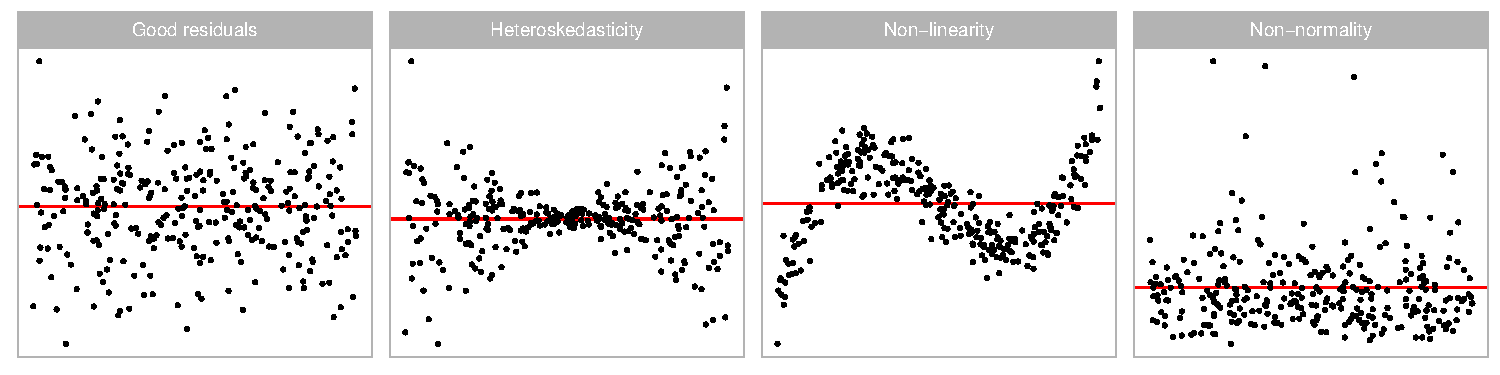
\includegraphics[width=1\linewidth]{paper_comparison_files/figure-latex/residual-plot-common-departures-1} 

}

\caption{Example residual vs fitted value plots: (A) classically good looking residuals, (B) non-linear pattern indicates that the model has not captured a non-linear association, (C) heteroskedasticity indicating that variance around the fitted model is not uniform, and (D) non-normality where the residual distribution is not symmetric around 0. The latter pattern might best be assessed using a univariate plot of the residuals, but patterns B and C need to be assessed using a residual vs fitted value plot.}\label{fig:residual-plot-common-departures}
\end{figure}

Graphical summaries in which residuals are plotted against fitted values
or other functions of the predictors that are approximately orthogonal
to residuals are referred to as standard residual plots in
\citet{cook1982residuals}. The first panel of Figure
\ref{fig:residual-plot-common-departures} shows an ideal residual plot
with residuals evenly distributed at both sides of the horizontal zero
line, with no noticeable patterns.

There are various types of departures from an ideal residual plot.
Non-linearity, heterskedasticity and non-normality are perhaps the three
mostly checked departures.

Non-linearity is a type of model misspecification caused by failing to
include higher order terms of the predictors in the regression equation.
Any non-linear functional form of residuals on fitted values in the
residual plot could be indicative of non-linearity. An example residual
plot containing visual pattern of non-linearity is given at the second
panel of Figure \ref{fig:residual-plot-common-departures}. One can
clearly observe the ``S-shape'' from the residual plot as the cubic term
is not captured by the misspecified model.

Heteroskedasticity refers to the presence of nonconstant error variance
in a regression model. It is mostly due to the strict but false
assumptions on the variance-covariance matrix of the error term. The
usual pattern of heteroskedasticity on a residual plot is the
inconsistent spread of the residuals across the horizontal axis.
Visually, it sometimes results in the so-called ``butterfly'' shape as
shown in the third panel of Figure
\ref{fig:residual-plot-common-departures}, or the ``left-triangle'' and
``right-triangle'' shape where the smallest variance occurs at one side
of the horizontal axis.

Compared to non-linearity and heteroskedasticity, non-normality is
usually harder to detect from a residual plot since a scatter plot do
not readily reveal the marginal distribution. A favourable graphical
summary for this task is the quantile-quantile plot. As we mainly
discuss residual plots, non-normality will not be the focus of this
paper. For a consistent comparison, the residual plot of this departure
is still presented in the fourth panel of Figure
\ref{fig:residual-plot-common-departures}. When the number residuals
below and above the horizontal axis are uneven across the local regions
along the \(x\)-axis, we expect that the normality assumption is
violated. For example, given a skewed error distribution, there will be
fewer data points and more outliers on one side of the horizontal axis
as shown in the fourth panel of Figure
\ref{fig:residual-plot-common-departures}.

\hypertarget{conventionally-testing-for-departures}{%
\subsection{Conventionally testing for
departures}\label{conventionally-testing-for-departures}}

Other than checking diagnostic plots, analysts may perform formal
hypothesis testing for detecting model defects. Depending on the
alternative hypothesis that is focused on, a variety of tests can be
applied. For example, the presence of heteroskedasticity can usually be
tested by applying the White test
\citep{white_heteroskedasticity-consistent_1980} or the Breusch-Pagan
test \citep{breusch_simple_1979}, which are both derived from the
Lagrange multiplier test \citep{silvey1959lagrangian} principle that
relies on the asymptotic properties of the null distribution. For
testing non-linearity, one may apply the F-test as a model structural
test to examine the significance of specific polynomial and non-linear
forms of the predictors, or the significance of proxy variables as in
the Ramsey Regression Equation Specification Error Test (RESET)
\citep{ramsey_tests_1969}. The Shapiro-Wilk test
\citep{shapiro1965analysis} is the most widely used test of
non-normality included by many of the statistical softwares. The
Jarque--Bera test \citep{jarque1980efficient} is also used to directly
checks if the sample skewness and kurtosis match a normal distribution.

Example residual plots given in Figure
\ref{fig:residual-plot-common-departures} are examined by the
corresponding RESET test, Breusch-Pagan test and Shapiro-Wilk test as
shown in Table \ref{tab:example-residual-plot-table}. In the example,
the Breusch-Pagan test and the Shapiro--Wilk test both reject \(H_0\)
for departures that they do not intend to examine. As discussed in
\citet{cook1982residuals}, most residual-based tests for a particular
type of departure from model assumptions are also sensitive to other
types of departures. It is likely \(H_0\) is correctly rejected but for
the wrong reason, a phenomenon known as the ``Type III error''.
Additionally, outliers will often incorrectly trigger the rejection of
\(H_0\) despite when majority of the residuals are well-behaved
\citep{cook_applied_1999}. Furthermore, with a sufficiently large sample
size, residual-based tests may reject \(H_0\) due to a slight departure
that is of little practical significance. These can be largely avoided
in diagnostic plots as experienced analysts can evaluate the
acceptability of assumptions flexibly, even in the presence of outliers
and slight departures.

\begin{table}

\caption{\label{tab:example-residual-plot-table}Statistical significance testing for departures from good residuals for plots in Figure \ref{fig:residual-plot-common-departures}. Shown are the $p$-values calculated for the RESET, the Breusch-Pagan and the Shapiro–Wilk tests. The good residual plot (A) is judged a good residual plot, as expected, by all tests. The non-linearity (B) is detected by all tests, as might be expected given the extreme structure.}
\centering
\begin{tabular}[t]{llrrr}
\toprule
Plot & Departures & RESET & Breusch-Pagan & Shapiro–Wilk\\
\midrule
A & None & 0.779 & 0.133 & 0.728\\
B & Non-linearity & \em{0.000} & \em{0.000} & \em{0.039}\\
C & Heteroskedasticity & 0.658 & \em{0.000} & \em{0.000}\\
D & Non-normality & 0.863 & 0.736 & \em{0.000}\\
\bottomrule
\end{tabular}
\end{table}

\hypertarget{visual-test-procedure-based-on-lineups}{%
\subsection{Visual test procedure based on
lineups}\label{visual-test-procedure-based-on-lineups}}

One may argue that reading diagnostic plots is to some extent subjective
and indecisive compared to those rigorous statistical procedures as it
relies on graphical perception - human ability to interpret and decode
the information embedded in graph \citep{cleveland_graphical_1984}.
Further, the degree of the presence of the visual features typically can
not be measured quantitatively and objectively, which may lead to over
or under-interpretations of the data. For instance, people
over-interpret the separation between gene groups in a two-dimensional
projection from a linear discriminant analysis when in fact there are no
differences in the expression levels between the gene groups and
separation is not an uncommon occurrence
\citep{roy_chowdhury_using_2015}.

Visual inference was first introduced in a 1999 Joint Statistical
Meetings (JSM) talk with the title ``Inference for Data Visualization''
by \citet{buja_inference_1999} as an idea to address the issue of valid
inference for visual discoveries of data plots. Later,
\citet{buja_statistical_2009} proposed the lineup protocol as a visual
test inspired by the ``police lineup'' or ``identity parade'' which is
the act of asking the eyewitness to identify criminal suspect from a
group of irrelevant people. The protocol consists of \(m\) randomly
placed plots, where one plot is the data plot, and the remaining
\(m - 1\) null plots have the identical graphical procedure except the
data has been replaced with data consistent with \(H_0\), that the model
is correctly specified. Then, an observer who have not seen the data
plot will be asked to point out the most different plot from the lineup.
Under \(H_0\), it is expected that the data plot would have no
distinguishable difference from the null plots, and the probability that
the observer correctly picks the data plot is \(1/m\). If one rejects
\(H_0\) as the observer correctly picks the data plot, then the Type I
error of this test is \(1/m\).

\begin{figure}

{\centering 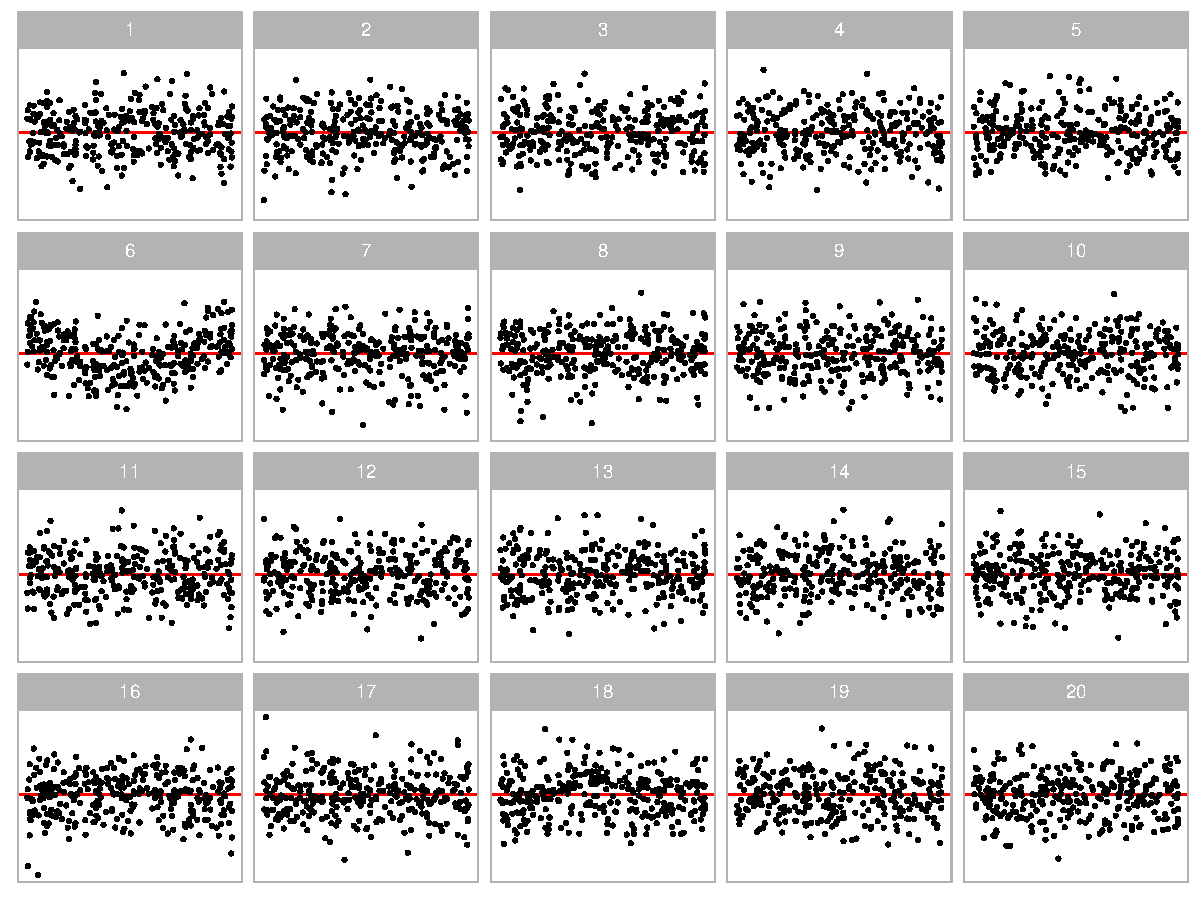
\includegraphics[width=1\linewidth]{paper_comparison_files/figure-latex/first-example-lineup-1} 

}

\caption{Visual testing is conducted using a lineup, as in the example here. The residual plot computed from the observed data (plot $2^2 + 2$, exhibiting non-linearity) is embedded among 19 null plots, where the residuals are simulated from a standard error model. Computing the $p$-value requires that the lineup be examined by a number of human judges, each asked to select the most different plot. A small $p$-value would result from a substantial number selecting plot $2^2 + 2$.}\label{fig:first-example-lineup}
\end{figure}

Figure \ref{fig:first-example-lineup} is an example of a lineup
protocol. If the data plot at position \(2^2 + 2\) is identifiable, then
it is evidence for the rejection of \(H_0\). In fact, the actual
residual plot is obtained from a misspecified regression model with
missing non-linear terms.

Data used in the \(m - 1\) null plots needs to be simulated. In
regression diagnostics, sampling data consistent with \(H_0\) is
equivalent to sampling data from the assumed model. As
\citet{buja_statistical_2009} suggested, \(H_0\) is usually a composite
hypothesis controlled by nuisance parameters. Since regression models
can have various forms, there is no general solution to this problem,
but it sometimes can be reduced to a so called ``reference
distribution'' by applying one of the three methods: (i) sampling from a
conditional distribution given a minimal sufficient statistic under
\(H_0\), (ii) parametric bootstrap sampling with nuisance parameters
estimated under \(H_0\), and (iii) Bayesian posterior predictive
sampling. The conditional distribution given a minimal sufficient
statistic is the best justified reference distribution among the three
\citep{buja_statistical_2009}. Essentially, null residuals can be
simulated by regressing \(N\) i.i.d standard normal random draws on the
predictors, then rescaling it by the ratio of residual sum of square in
two regressions.

The effectiveness of lineup protocol for regression analysis is
validated by \citet{majumder_validation_2013} under relatively simple
settings with up to two predictors. Their results suggest that visual
tests are capable of testing the significance of a single predictor with
a similar power as a t-test, though they express that in general it is
unnecessary to use visual inference if there exists a conventional test,
and they do not expect the visual test to perform equally well as the
conventional test. In their third experiment, where there is not a
conventional test, visual test outperforms the conventional test for a
large margin. This is encouraging, as it promotes the use of visual
inference in situations where there are no existing statistical testing
procedures. Visual inference have also been integrated into diagnostic
of hierarchical linear models by \citet{loy2013diagnostic},
\citet{loy2014hlmdiag} and \citet{loy2015you}. They use lineup protocols
to judge the assumption of linearity, normality and constant error
variance for both the level-1 and level-2 residuals. (expand?)

\hypertarget{calculation-of-statistical-significance-and-test-power}{%
\section{Calculation of statistical significance and test
power}\label{calculation-of-statistical-significance-and-test-power}}

\hypertarget{what-is-being-tested}{%
\subsection{What is being tested?}\label{what-is-being-tested}}

In diagnosing a model fit from residuals, we are generally interested in
\(H_0:\) \emph{The regression model is correctly specified} against the
broad alternative \(H_a:\) \emph{The regression model is misspecified}.

However, it is practically impossible to test this specific \(H_0\) with
conventional tests, which are constructed to measure specific
departures. For example, the RESET test is formulated as
\(H_0:\gamma_1 = \gamma_2 = \gamma_3 = 0\) against
\(H_a: \gamma_1 \neq 0 \text{ or } \gamma_2 \neq 0 \text{ or } \gamma_3 \neq 0\),
from
\(e = \tau_0 + \tau_1x_1 + ... + \tau_1 x_p +\gamma_1\hat{y}^2 + \gamma_2\hat{y}^3 + \gamma_3\hat{y}^4 + u, ~~u \sim N(0, \sigma_u^2)\).
Similarly, the Breusch-Pagan test is designed to specifically test
\(H_0:\) \emph{error variances are all equal}
(\(\tau_i=0 \text{ for } i=1,..,p\)) versus the alternative \(H_a:\)
\emph{that the error variances are a multiplicative function of one or
more variables} (\(\text{at least one } \tau_i\neq 0\)) from
\(e^2 = \tau_0 + \tau_1 x_1 + \cdots + \tau_1 x_p + u, ~ u\sim N(0,\sigma_u^2)\).

One of the potential benefits of the visual test, based on the lineup
protocol, is that it should be able to detect a range of departures from
good residuals.

\hypertarget{statistical-significance}{%
\subsection{Statistical significance}\label{statistical-significance}}

In hypothesis testing, a \(p\)-value is defined as the probability of
observing test results as least as extreme as the observed result given
\(H_0\) is true. Conventional hypothesis tests usually have an existing
method to derive or compute \(p\)-value based on the null distribution.
What we need to discuss in the following is the method to estimate
\(p\)-value for a visual test.

Within the context of visual inference, by involving \(k\) independent
observers, the visual \(p\)-value can be interpreted as the probability
of having as many or more subjects detect the data plot than the
observed result.

Let \(X_j = \{0,1\}\) be a Bernoulli random variable denoting whether
subject \(j\) correctly detecting the data plot, and
\(X = \sum_{j=1}^{K}X_j\) be the number of observers correctly picking
the data plot. Then, by imposing a relatively strong assumption on the
visual test that all \(K\) evaluations are fully independent, under
\(H_0\), \(X \sim \mathrm{Binom}_{K,1/m}\). Therefore, the \(p\)-value
of a lineup of size \(m\) evaluated by \(K\) observer is given as
\(P(X \geq x) = 1 - F(x) + f(x)\), where \(F(.)\) is the binomial
cumulative distribution function, \(f(.)\) is the binomial probability
mass function and \(x\) is the realization of number of observers
correctly picking the data plot \citep{majumder_validation_2013}.

As pointed out by \citet{vanderplas2021statistical}, this basic binomial
model doesn't take into account the possible dependencies in the visual
test due to repeated evaluations of the same lineup. And it is
inapplicable to visual test where subjects are asked to select one or
more ``most different'' plots from the lineup.
\citet{vanderplas2021statistical} summarises three common scenarios in
visual inference: (1) \(K\) different lineups are shown to \(K\)
subjects, (2) \(K\) lineups with different null plots but the same data
plot are shown to \(K\) subjects, and (3) the same lineup is shown to
\(K\) subjects. Out of these three scenarios, Scenario 3 is the most
common in previous studies as it puts the least constraints on the
experiment design. For Scenario 3, \citet{vanderplas2021statistical}
models the probability of a plot \(i\) being selected from a lineup as
\(\theta_i\), where \(\theta_i \sim Dirichlet(\alpha)\) for
\(i=1,...,m\) and \(\alpha > 0\). The number of times plot \(i\) being
selected in \(K\) evaluations is denoted as \(c_i\). In case subject
\(j\) makes multiple selections, \(1/s_j\) will be added to \(c_i\)
instead of one, where \(s_j\) is the number of plots subject \(j\)
selected for \(j=1,...K\). This ensures \(\sum_{i}c_i=K\). Since we are
only interested in the selections of the data plot \(i\), the marginal
model can be simplified to a beta-binomial model and thus the visual
p-value is given as

\begin{equation} \label{eq:pvalue-beta-binomial}
P(C \geq c_i) = \sum_{x=c_i}^{K}{K \choose x}\frac{B(x + \alpha, K - x + (m - 1)\alpha)}{B(\alpha, (m-1)\alpha)},\quad \text{for} \quad c_i \in \mathbb{Z}_0^+
\end{equation}

\noindent where \(B(.)\) is the beta function defined as

\begin{equation} \label{eq:betafunction}
B(a, b) = \int_{0}^{1}t^{\alpha - 1}(1-t)^{b-1}dt,\quad \text{where}\quad a,b>0.
\end{equation}

Note that Equation \ref{eq:pvalue-beta-binomial} given in
\citet{vanderplas2021statistical} only works with non-negative integer
\(c_i\). We extend the equation to non-negative real number \(c_i\) by
applying a linear approximation

\begin{equation} \label{eq:pvalue-beta-binomial-approx}
P(C \geq c_i) = P(C \geq \lceil c_i \rceil) + (\lceil c_i \rceil - c_i) P(C = \lfloor c_i \rfloor), \quad \text{for}\quad c_i \in \mathbb{R}_0^+,
\end{equation}

where \(P(C \geq \lceil c_i \rceil)\) is calculated using Equation
\ref{eq:pvalue-beta-binomial} and \(P(C = \lfloor c_i \rfloor)\) is
calculated by

\begin{equation} \label{eq:pmf-beta-binomial}
P(C = c_i) = {K \choose c_i}\frac{B(c_i + \alpha, K - c_i + (m - 1)\alpha)}{B(\alpha, (m-1)\alpha)},\quad \text{for} \quad c_i \in \mathbb{Z}_0^+.
\end{equation}

Besides, the parameter \(\alpha\) used in Equation
\ref{eq:pvalue-beta-binomial} and \ref{eq:pmf-beta-binomial} is usually
unknown and hence needs to be estimated from the survey data. For low
values of \(\alpha\), only a few plots are attractive to the observers
and tend to be selected. For higher values of \(\alpha\), the
distribution of the probability of each plot being selected is more
even. \citet{vanderplas2021statistical} defines that a plot is
\(c\)-interesting if \(c\) or more participants select the plot as the
most different. Given the definition, The expected number of plots
selected at least \(c\) times, \(E[Z_c]\), is calculated as

\begin{equation} \label{eq:c-interesting-expectation}
E[Z_c(\alpha)] = \frac{m}{B(\alpha, (m-1)\alpha)}\sum_{\lceil c \rceil}^{K}{K \choose x} B(x + \alpha, K - x + (m-1)\alpha).\end{equation}

With Equation \ref{eq:c-interesting-expectation}, \(\alpha\) can be
estimated using maximum likelihood estimation. But for precise estimate
of \(\alpha\), additional human responses to Rorschach lineups, which is
a type of lineup that consists of plots constructed from the same null
data generating mechanism, are required.

\hypertarget{power-of-the-tests}{%
\subsection{Power of the tests}\label{power-of-the-tests}}

The power of a model misspecification test is the probability that
\(H_0\) is rejected given the regression model is misspecified in a
specific way. It is an important indicator when one is concerned about
whether model assumptions have been violated. Although in practice, one
might be more interested in knowing how much the residuals deviate from
the model assumptions, and whether this deviation is of practical
significance.

The power of a conventional hypothesis test is affected by both the true
parameter \(\boldsymbol{\theta}\) and the sample size \(n\). These two
can be quantified in terms of effect size \(E\) to measure the strength
of the residual departures from the model assumptions. Details about the
effect size is provided in Section \ref{effect-size} after the
introduction of the simulation model used in our human subject
experiment. The theoretical power of a test is sometimes not a trival
solution, but it can be estimated if the data generating process is
known. We use a predefined model to generate a large set of simulated
data under different effect sizes, and record if the conventional test
rejects \(H_0\). The probability of the conventional test rejects
\(H_0\) is then fitted by a logistic regression formulated as

\begin{equation} \label{eq:logistic-regression-1-1}
Pr(\text{reject}~H_0|H_1,E) = \Lambda\left(log\left(\frac{0.05}{0.95}\right) + \beta_1 E\right),
\end{equation}

\noindent where \(\Lambda(.)\) is the standard logistic function given
as \(\Lambda(z) = exp(z)/(1+exp(z))\). The effect size \(E\) is the only
predictor and the intercept is fixed to \(log(0.05/0.95)\) so that
\(\hat{Pr}(\text{reject}~H_0|H_1,E = 0) = 0.05\), which is the desired
significance level.

The power of a visual test on the other hand, may additionally depend on
the ability of the particular subject, as the skill of the individual
may affect the number of observers who identify the data plot from the
lineup \citep{majumder_validation_2013}. To address this issue,
\citet{majumder_validation_2013} models the probability of a subject
\(j\) correctly picking the data plot from a lineup \(l\) using a
mixed-effect logistic regression, with subjects treated as random
effect. Then, the estimated power of a visual test evaluated by a single
subject is the predicted value obtained from the mix-effect model.
However, this mix-effect model does not work with scenario where
subjects are asked to select one or more most different plots. In this
scenario, having the probability of a subject \(j\) correctly picking
the data plot from a lineup \(l\) is insufficient to determine the power
of a visual test because it does not provide information about the
number of selections made by the subject for the calculation of the
p-value (See Equation \ref{eq:pvalue-beta-binomial-approx}). Therefore,
we directly estimate the probability of a lineup being rejected by
assuming that individual skill has negligible effect on the variation of
the power. This assumption is not necessary true, but it helps
simplifying the model structure, thereby obviate a costly large-scale
experiment to estimate complex covariance matrices. The same model given
in Equation \ref{eq:logistic-regression-1-1} is applied to model the
power of a visual test.

To study various factors contributing to the power of both tests, the
same logistic regression model is fit on different subsets of the
collated data grouped by levels of factors. These include the
distribution of the fitted values, type of the simulation model and the
shape of the residual departures.

\hypertarget{experimental-design}{%
\section{Experimental design}\label{experimental-design}}

An experiment is conducted in three data collection periods to
investigate the difference between conventional hypothesis testing and
visual inference in the application of linear regression diagnostics.
Two types of departures, non-linearity and heteroskedasticity, are
collected during data collection periods I and II. The data collection
period III was designed primarily to measure human responses to null
lineups so that the parameter \(\alpha\) in Equation
\ref{eq:pvalue-beta-binomial} can be estimated. Additional lineups for
both non-linearity and heteroskedasticity, using uniform fitted value
distribution, were included so that the participants were evaluating
some lineups with signal also. It would be too frustrating for
participants to only be assigned lineups with all null plots. Overall,
we collected 7974 evaluations on 1152 unique lineups performed by 443
subjects throughout three data collection periods.

\hypertarget{simulating-departures-from-good-residuals}{%
\subsection{Simulating departures from good
residuals}\label{simulating-departures-from-good-residuals}}

\hypertarget{non-linearity}{%
\subsubsection{Non-linearity}\label{non-linearity}}

Data collection period I is designed to study the ability of human
subjects to detect the effect of a non-linear term \(\boldsymbol{z}\)
constructed using Hermite polynomials on random vector
\(\boldsymbol{x}\) formulated as

\begin{align} \label{eq:nonlinearity-model}
\boldsymbol{y} &= 1 + \boldsymbol{x} + \boldsymbol{z} + \boldsymbol{\varepsilon},\\
\boldsymbol{x} &= g(\boldsymbol{x}_{raw}, 1), \\
\boldsymbol{z} &= g(\boldsymbol{z}_{raw}, 1), \\
\boldsymbol{z}_{raw} &= He_j(g(\boldsymbol{x}, 2)),
\end{align}

\noindent where \(\boldsymbol{y}\), \(\boldsymbol{x}\),
\(\boldsymbol{\varepsilon}\), \(\boldsymbol{x}_{raw}\),
\(\boldsymbol{z}_{raw}\) are vectors of size \(n\), \(He_{j}(.)\) is the
\(j\)th-order probabilist's Hermite polynomials,
\(\varepsilon \sim N(\boldsymbol{0}, \sigma^2\boldsymbol{I}_n)\), and
\(g(\boldsymbol{x}, k)\) is a scaling function to enforce the support of
the random vector to be \([-k, k]^n\) defined as

\begin{equation} \label{eq:scaling-function}
g(\boldsymbol{x}, k) = (\boldsymbol{x} - min(\boldsymbol{x}))/max(\boldsymbol{x} - min(\boldsymbol{x}))2k - k, \quad \text{for} \quad k > 0. 
\end{equation}

According to \citet{abramowitz1964handbook}, Hermite polynomials were
initially defined by \citet{de1820theorie}, but named after Hermite
\citep{hermite1864nouveau} because of the unrecognisable form of
Laplace's work. When simulating \(\boldsymbol{z}_{raw}\), function
\texttt{hermite} from the R package \texttt{mpoly} \citep{mpoly} is used
to generate Hermite polynomials.

The null regression model used to fit the realizations generated by the
above model is formulated as

\begin{equation} \label{eq:null-model}
\boldsymbol{y} = \beta_0 + \beta_1 \boldsymbol{x} + \boldsymbol{u},
\end{equation}

\noindent where
\(\boldsymbol{u} \sim N(\boldsymbol{0}, \sigma^2\boldsymbol{I}_n)\).

Since \(z = O(x^j)\), for \(j > 1\), \(z\) is a higher order term leaves
out by the null regression, which will lead to model misspecification.

Visual patterns of non-linearity are simulated using four different
orders of probabilist's Hermite polynomials (\(j = 2, 3, 6, 18\)). (A
summary of the factors is given in Table \ref{tab:model-factor-table}.)
The values of \(j\) is chosen so that distinct shapes of non-linearity
are included in the residual plot. These include ``U'', ``S'', ``M'' and
``Triple-U'' shape as shown in Figure
\ref{fig:different-shape-of-herimite}. A greater value of \(j\) will
result in a curve with more turning points. It is expected that the
``U'' shape will be the easiest one to detect because complex shape
tends to be concealed by cluster of data points.

Figure \ref{fig:example-poly-lineup} demonstrates one of the lineups
used in non-linearity detection. This lineup is produced by the
non-linearity model with \(j = 6\). The data plot location is
\(2^3 - 4\). All five subjects correctly identify the data plot from
this lineup.

\begin{table}

\caption{\label{tab:model-factor-table}Levels of the factors used in data collection periods I, II, III.}
\centering
\resizebox{\linewidth}{!}{
\begin{tabular}[t]{rr|rr|rcrr|rr|rcrr|rr|rcrr|rr|rcrr|rr|rcrr|rr|rc}
\toprule
\multicolumn{2}{c}{Non-linearity} & \multicolumn{2}{c}{Heteroskedasticity} & \multicolumn{2}{c}{Common} \\
\cmidrule(l{3pt}r{3pt}){1-2} \cmidrule(l{3pt}r{3pt}){3-4} \cmidrule(l{3pt}r{3pt}){5-6}
\multicolumn{1}{c}{Poly Order ($j$)} & \multicolumn{1}{c}{SD ($\sigma$)} & \multicolumn{1}{c}{Shape ($a$)} & \multicolumn{1}{c}{Ratio ($b$)} & \multicolumn{1}{c}{Size ($n$)} & \multicolumn{1}{c}{Distribution of fitted values} \\
\cmidrule(l{3pt}r{3pt}){1-1} \cmidrule(l{3pt}r{3pt}){2-2} \cmidrule(l{3pt}r{3pt}){3-3} \cmidrule(l{3pt}r{3pt}){4-4} \cmidrule(l{3pt}r{3pt}){5-5} \cmidrule(l{3pt}r{3pt}){6-6}
2 & 0.25 & -1 & 0.25 & 50 & Uniform\\
3 & 1.00 & 0 & 1.00 & 100 & Normal\\
6 & 2.00 & 1 & 4.00 & 300 & Skewed\\
18 & 4.00 &  & 16.00 &  & Discrete uniform\\
 &  &  & 64.00 &  & \\
\bottomrule
\end{tabular}}
\end{table}

\begin{figure}

{\centering 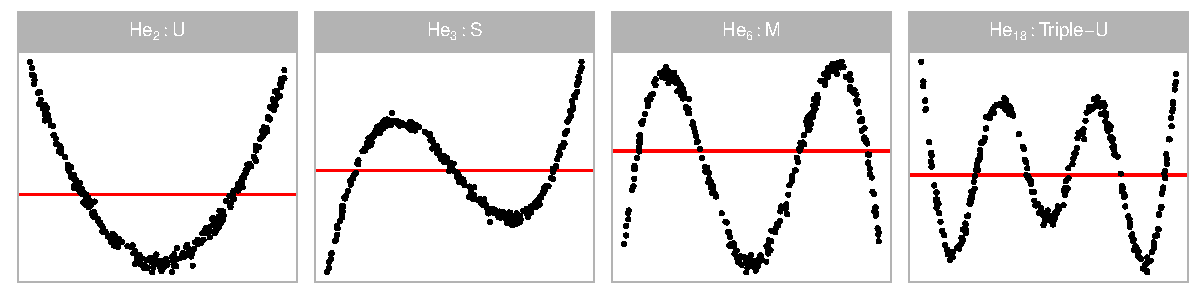
\includegraphics[width=1\linewidth]{paper_comparison_files/figure-latex/different-shape-of-herimite-1} 

}

\caption{Polynomial forms generated for the residual plots used to assess detecting non-linearity. The four shapes are generated by varying the order of polynomial given by $j$ in $He_j(.)$.}\label{fig:different-shape-of-herimite}
\end{figure}

\begin{figure}

{\centering 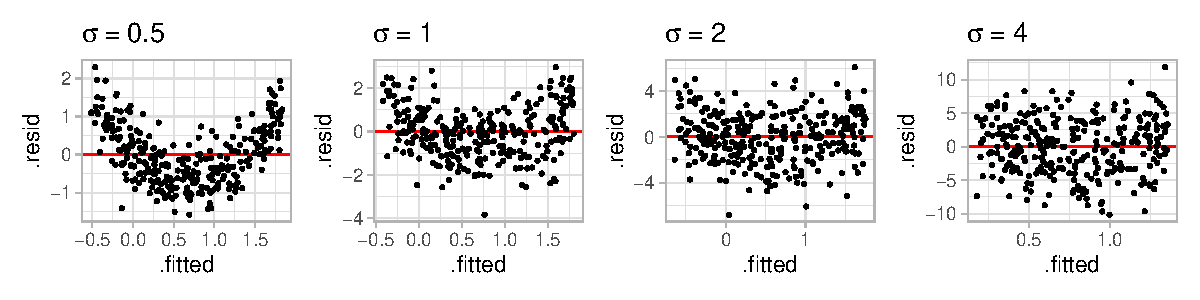
\includegraphics[width=1\linewidth]{paper_comparison_files/figure-latex/different-sigma-1} 

}

\caption{Examining the effect of $\sigma$ on the signal strength in the non-linearity detection, for $n=300$, uniform fitted value distribution and the U shape. As $\sigma$ increases the signal strength decreases, to the point that the U is almost unrecognisable when $\sigma=4$.}\label{fig:different-sigma}
\end{figure}

\begin{figure}

{\centering 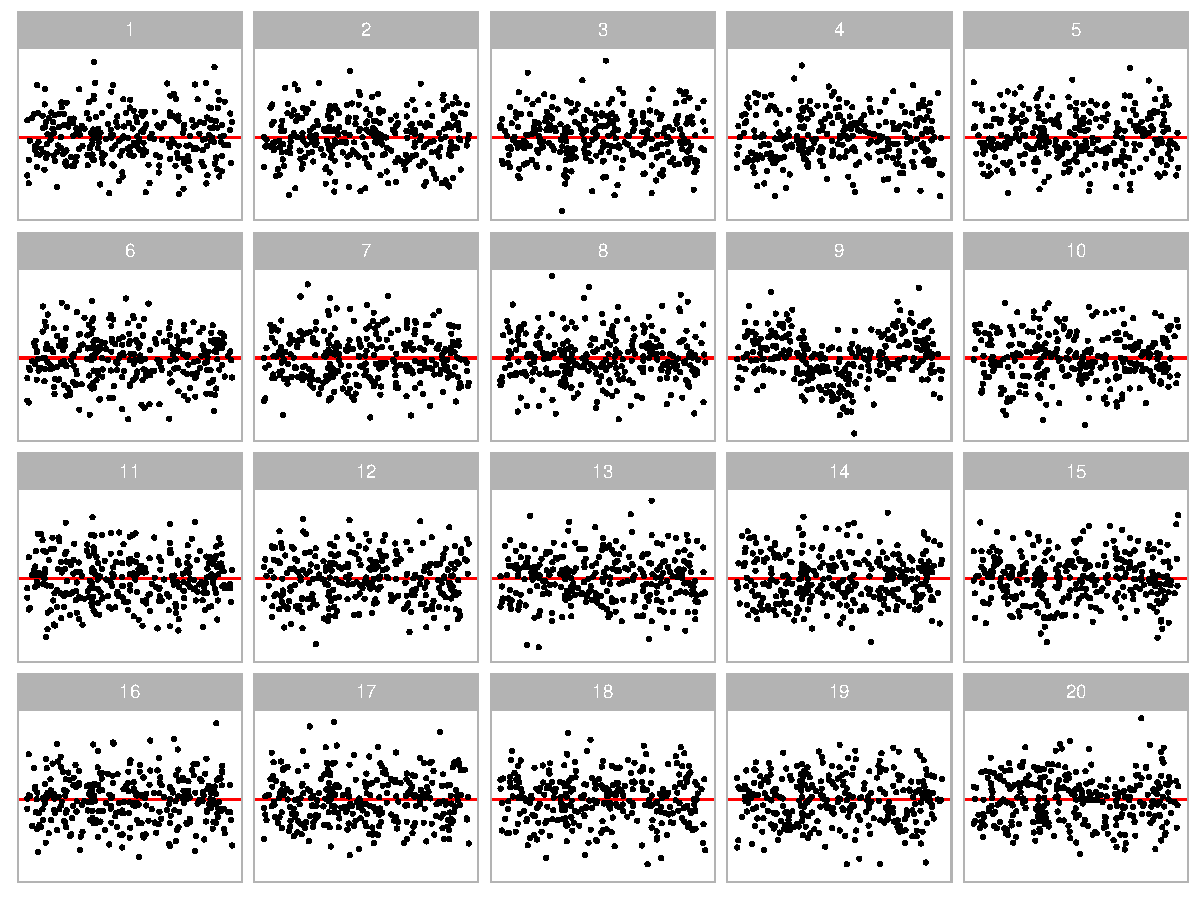
\includegraphics[width=1\linewidth]{paper_comparison_files/figure-latex/example-poly-lineup-1} 

}

\caption{One of the lineups containing non-linearity patterns used in data collection period I. Can you spot the most different plot? The data plot is positioned at $2^3 + 1$.}\label{fig:example-poly-lineup}
\end{figure}

\hypertarget{heteroskedasticity}{%
\subsubsection{Heteroskedasticity}\label{heteroskedasticity}}

Data collection period II is designed to study the ability of human
subjects to detect the appearance of a heteroskedasticity pattern under
a simple linear regression model setting:

\begin{align} \label{eq:heter-model}
\boldsymbol{y} &= 1 + \boldsymbol{x} + \boldsymbol{\varepsilon},\\
\boldsymbol{x} &= g(\boldsymbol{x}_{raw}, 1),\\
\boldsymbol{\varepsilon} &\sim N(\boldsymbol{0}, 1 + (2 - |a|)(\boldsymbol{x} - a)^2b \boldsymbol{I}), 
\end{align}

\noindent where \(\boldsymbol{y}\), \(\boldsymbol{x}\),
\(\boldsymbol{\varepsilon}\) are vectors of size \(n\) and \(g(.)\) is
the scaling function defined in Equation \ref{eq:scaling-function}.

The null regression model used to fit the realizations generated by the
above model is formulated exactly the same as Equation
\ref{eq:null-model}.

For \(b \neq 0\), the variance-covariance matrix of the error term
\(\boldsymbol{\varepsilon}\) is correlated with the predictor
\(\boldsymbol{x}\), which will lead to the presence of
heteroskedasticity. Visual patterns of heteroskedasticity are simulated
using three different shapes (\(a\) = -1, 0, 1). (A summary of the
factors can be found in Table \ref{tab:model-factor-table}.)

Since \(supp(X) = [-1, 1]\), choosing \(a\) to be \(-1\), \(0\) and
\(1\) can generate ``left-triangle'', ``butterfly'' and
``right-triangle'' shape as displayed in Figure
\ref{fig:different-shape-of-heter}. The term \((2 - |a|)\) maintains the
magnitude of residuals across different values of \(a\).

\begin{figure}

{\centering 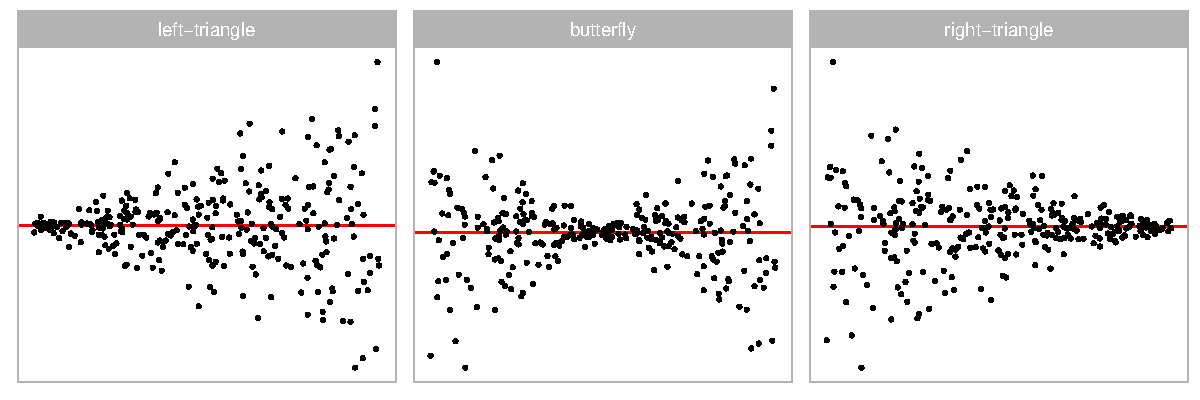
\includegraphics[width=1\linewidth]{paper_comparison_files/figure-latex/different-shape-of-heter-1} 

}

\caption{Heteroskedasticity forms used in the experiment. Three different shapes ($a = -1, 0, 1$) are used in the experiment to create left-triangle, butterfly and right-triangle shapes, respectively.}\label{fig:different-shape-of-heter}
\end{figure}

\begin{figure}

{\centering 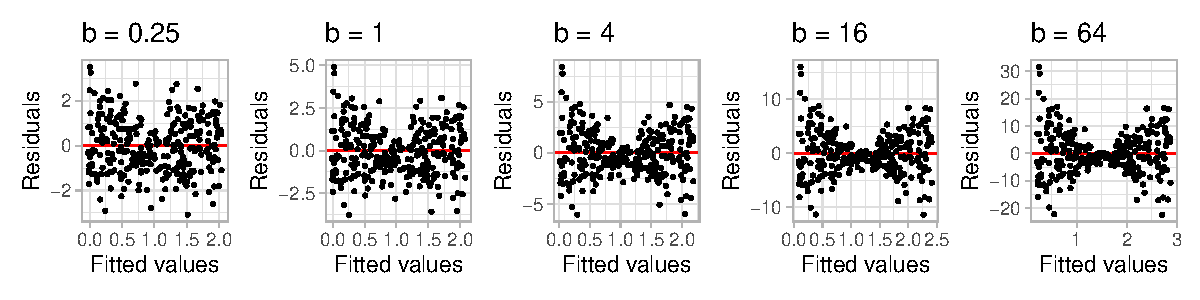
\includegraphics[width=1\linewidth]{paper_comparison_files/figure-latex/different-b-1} 

}

\caption{Five different values of $b$ are used in heteroskedasticity simulation to control the strength of the signal. Larger values of $b$ yield a bigger difference in variation, and stus stronger heteroskedasticity signal.}\label{fig:different-b}
\end{figure}

\begin{figure}

{\centering 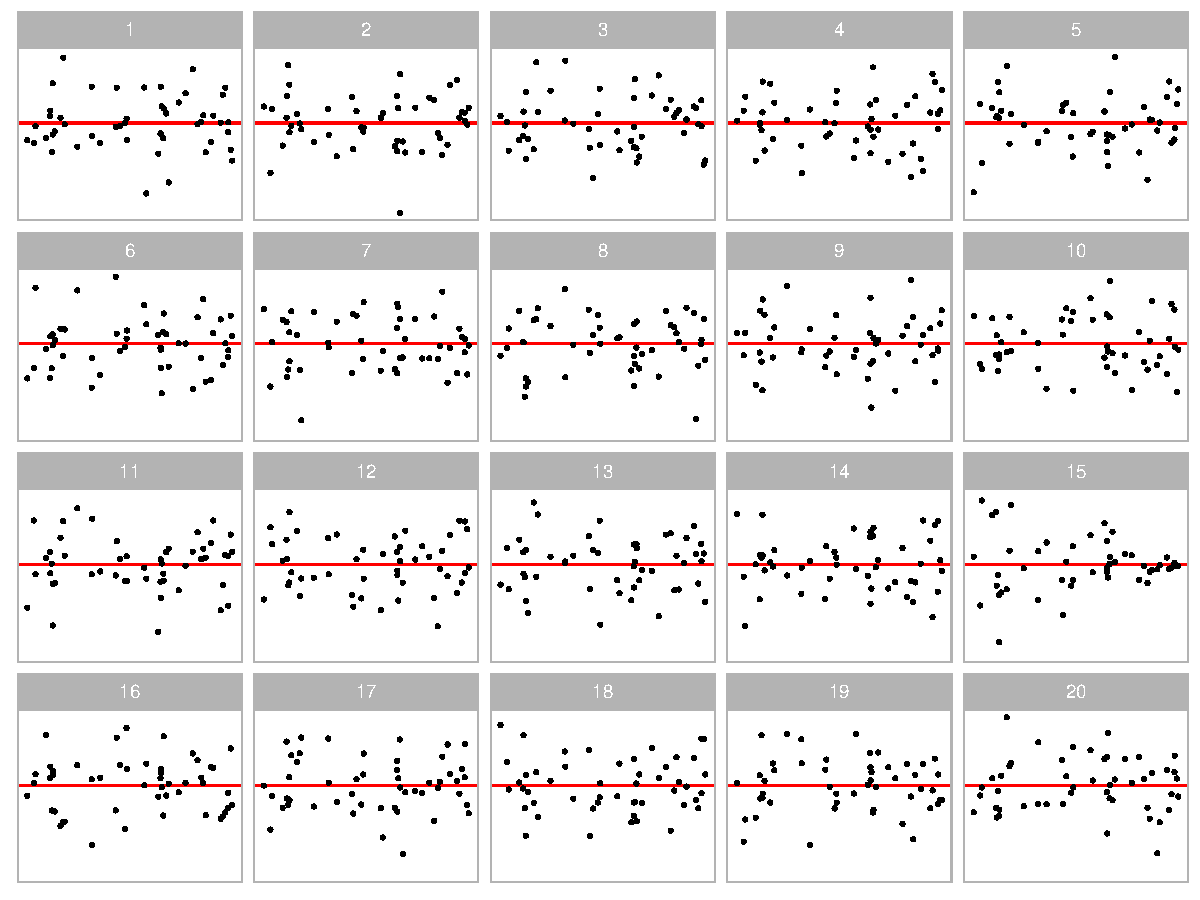
\includegraphics[width=1\linewidth]{paper_comparison_files/figure-latex/example-heter-lineup-1} 

}

\caption{One of the lineups containing heteroskedasticity pattern used in data collection period II. Can you spot the most different plot? The data plot is positioned at $3^3 - 3^2$}\label{fig:example-heter-lineup}
\end{figure}

An example lineup of this model used in data collection period II is
shown in Figure \ref{fig:example-heter-lineup} with \(a = -1\). The data
plot location is \(2^4 + 2\). Nine out of 11 subjects correctly identify
the data plot from this lineup.

\hypertarget{factors-common-to-both-data-collection-periods}{%
\subsubsection{Factors common to both data collection
periods}\label{factors-common-to-both-data-collection-periods}}

Fitted values are a function of the independent variables, and the
distribution of the observed values affects the distribution of the
fitted values. In the best case scenario the fitted values will have a
uniform distribution, which means that there is even coverage of
possible observed values across all of the predictors. This is not
always present in the collected data. Sometimes the fitted values are
discrete because one or more predictors were measured discretely. The
distribution may be relatively Gaussian, reflecting a linear combinatio
of many predictors, adhering to the Central Limit Theorem. It is also
common to see a skewed distribution of fitted values, if one or more of
the predictors has a skewed distribution. This latter problem is usually
corrected before modelling using a variable transformation. Our
simulation assess this by using four different distributions to
represent fitted values: (1) uniform, (2) normal, (3) skewed and (4)
discrete uniform. This is constructed by defining the raw predictor
\(X_{raw}\) in four corresponding distributions: (1) \(U(-1, 1)\), (2)
\(N(0, 0.3^2)\), (3) \(lognormal(0, 0.6^2)/3\) and (4) \(u\{1, 5\}\). We
would expect that the best reading of residual plots occurs when the
fitted values are uniformly distributed.

Three different sample sizes are used, \(n=50, 100, 300\) across the
experiments. We would expect considerable variation in the signal
strength in the simulated data plots with smaller \(n\). A sample size
of 300 is typically enough for structure to be visible in a scatter plot
reliably.

\begin{figure}

{\centering 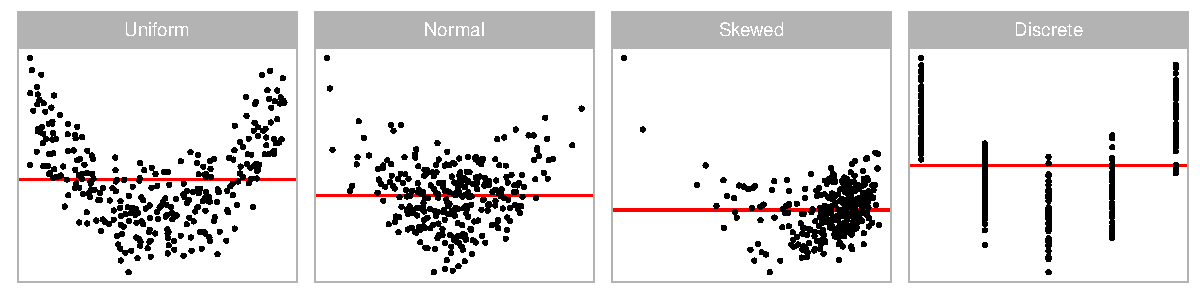
\includegraphics[width=1\linewidth]{paper_comparison_files/figure-latex/different-dist-1} 

}

\caption{Variations in fitted values, that might affect perception of residual plots. Four different distributions are used.}\label{fig:different-dist}
\end{figure}

\begin{figure}

{\centering 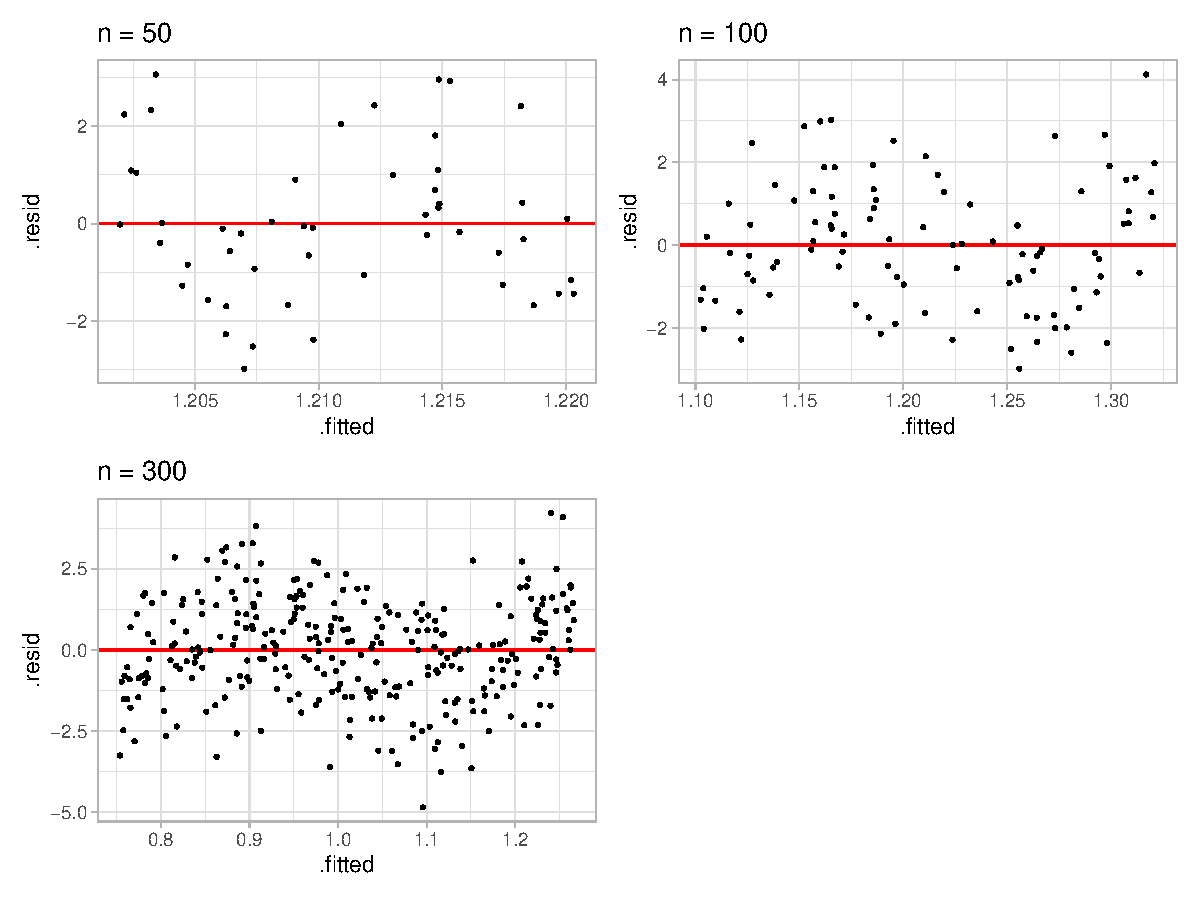
\includegraphics[width=1\linewidth]{paper_comparison_files/figure-latex/different-n-1} 

}

\caption{Examining the effect of signal strength for the three different values of $n$ used in the experiment, for non-linear structure with fixed $\sigma = 1.5$, uniform fitted value distribution, and S shape. For these factor levels, only when $n = 300$ is the S shape clearly visible.}\label{fig:different-n}
\end{figure}

\hypertarget{experimental-setup}{%
\subsection{Experimental setup}\label{experimental-setup}}

\hypertarget{controlling-the-strength-of-the-signal}{%
\subsubsection{Controlling the strength of the
signal}\label{controlling-the-strength-of-the-signal}}

As summarised in Table \ref{tab:model-factor-table}, three additional
parameters \(n\), \(\sigma\) and \(b\) are used to control the strength
of the signal so that different difficulty levels of lineups are
generated, and therefore, the estimated power curve will be smooth and
continuous. Parameter \(\sigma \in \{0.5, 1, 2, 4\}\) and
\(b \in \{0.25, 1, 4, 16, 64\}\) are used in data collection periods I
and II respectively. Figure \ref{fig:different-sigma} and
\ref{fig:different-b} demonstrate the impact of these two parameters. A
large value of \(\sigma\) will increase the variation of the error of
the non-linearity model and decrease the visibility of the visual
pattern. The parameter \(b\) controls the standard deviation of the
error across the support of the predictor. Given \(x \neq a\), a larger
value of \(b\) will lead to a larger ratio of the variance at \(x\) to
the variance at \(x - a = 0\), making the visual pattern more obvious.

Three different sample sizes are used (n = 50, 100, 300) in all three
data collection periods. It can be observed from Figure
\ref{fig:different-n} that with fewer data points drawn in a residual
plot, the visual pattern is more difficult to be detected.

\hypertarget{effect-size}{%
\subsubsection{Effect size}\label{effect-size}}

Effect size \(E\) can be defined as the difference of a parameter for a
particular model or distribution, or a statistic derived from a sample.
Importantly, it needs to reflect the treatment we try to measure.
According to the underlying simulated model, we define the effect size

\[E = \frac{1}{2}\left(\boldsymbol{\mu}_z'[diag(\boldsymbol{R}_a\sigma^2)]^{-1}\boldsymbol{\mu}_z\right)\]

for the non-linearity model, and

\[E = \frac{1}{2}\left(log\frac{|diag(\boldsymbol{R}_a\boldsymbol{V}\boldsymbol{R}_a')|}{|diag(\boldsymbol{R}_a)|} - n + tr(diag(\boldsymbol{R}_a\boldsymbol{V}\boldsymbol{R}_a')^{-1}diag(\boldsymbol{R}_a))\right)\]
for the heteroskedasticity model, where \(diag(.)\) is the diagonal
matrix constructed from the diagonal elements of a matrix,
\(\sigma^2\boldsymbol{I}\) is the assumed covariance matrix of the error
term when \(H_0\) is true, \(\boldsymbol{V}\) is the actual covariance
matrix of the error term,
\(\boldsymbol{R}_a = \boldsymbol{I}_n - \boldsymbol{H}_a\) is the
residual operator,
\(\boldsymbol{H}_a = \boldsymbol{X}_a(\boldsymbol{X}_a'\boldsymbol{X}_a)^{-1}\boldsymbol{X}_a'\)
is the hat matrix,
\(\boldsymbol{X}_a = (\boldsymbol{1}, \boldsymbol{X})\) is the matrix of
predictors including the intercept used in the regression equation, and
\(\boldsymbol{\mu}_z = \boldsymbol{R}_a\boldsymbol{Z}\boldsymbol{\beta}_z\)
is the expected values of residuals with \(\boldsymbol{Z}\) be any
higher order terms of \(\boldsymbol{X}\) leave out by the regression
equation and \(\boldsymbol{\beta}_z\) be the corresponding coefficients.

Both equations above are derived from the Kullback-Leibler divergence
(citation here?) and the details are provided in the Appendix.

\hypertarget{subject-allocation}{%
\subsubsection{Subject allocation}\label{subject-allocation}}

As shown in Table \ref{tab:model-factor-table}, there are a total of
\(4 \times 4 \times 3 \times 4 = 192\) and
\(3 \times 5 \times 3 \times 4 = 180\) number of combinations of
parameter values for non-linearity model and heteroskedasticity model
respectively. Three replications are made for each of the combination
results in \(192 \times 3 = 576\) and \(180 \times 3 = 540\) lineups. In
addition, each lineup is designed to be evaluated by five different
subjects. After attempting some pilot studies internally, we decide to
present a block of 20 lineups to every subject. And to ensure the
quality of the survey data, two lineups with obvious visual patterns are
included as attention checks. Thus, \(576 \times 5 / (20-2) = 160\) and
\(540 \times 5 / (20-2) = 150\) subjects are recruited to satisfy the
design of the data collection period I and II respectively.

As mentioned in Section \ref{power-of-the-tests}, \(\alpha\) used in
Equation \ref{eq:pvalue-beta-binomial} needs to be estimated using null
lineups. Three replications are made for \(3 \times 4 = 12\)
combinations of common factors \(n\) and fitted value distribution,
results in \(12 \times 3 = 36\) lineups included in data collection
period III. In these lineups, the data of the data plot is generated
from a model with zero effect size, while the data of the 19 null plots
are generated using the same simulation method discussed in Section
\ref{visual-test-procedure-based-on-lineups}. This generation procedure
differs from the canonical Rorschach lineup procedure, which requires
that all 20 plots are generated directly from the null model. However,
these lineups serve the same fundamental purpose: to assess the number
of visually interesting plots generated under \(H_0\).

To account for the fact that our simulation method for these lineups is
not the Rorschach procedure, we use the method suggested in
\citet{vanderplas2021statistical} for typical lineups containing a data
plot to estimate \(\alpha\). We have included a sensitivity analysis in
the Appendix to examine the impact of the variance of the \(\alpha\)
estimate on our findings.

All lineups consist of only null plots are planned to be evaluated by 20
subjects. However, presenting only these lineups to subjects are
considered to be bad practices as subjects will lose interest quickly.
Therefore, we plan to collect 6 more evaluations on the 279 lineups with
uniform fitted value distribution, result in
\((36 \times 20 + 279 \times 3 \times 6) / (20-2) = 133\) subjects
recruited for data collection period III.

\hypertarget{collecting-results}{%
\subsubsection{Collecting results}\label{collecting-results}}

Subjects for all three data collection periods are recruited from an
crowdsourcing platform called Prolific \citep{palan2018prolific}.
Prescreening procedure is applied during the recruitment, subjects are
required to be fluent in English, with \(98\%\) minimum approval rate
and 10 minimum submissions in other studies.

During the experiment, every subject is presented with a block of 20
lineups. A lineup consists of a randomly placed data plot and 19 null
plots, which are all residual plots drawn with raw residuals on the
y-axis and fitted values on the x-axis. An additional horizontal red
line is added at \(y = 0\) as a helping line.

The data of the data plot is simulated from one of two models described
in Section \ref{simulating-departures-from-good-residuals}, while the
data of the remaining 19 null plots are generated by the residual
rotation technique discussed in Section
\ref{visual-test-procedure-based-on-lineups}.

In every lineup evaluation, the subject is asked to select one or more
plots that are most different from others, provide a reason for their
selections, and evaluate how different they think the selected plots are
from others. If there is no noticeable difference between plots in a
lineup, subjects are permitted to select zero plots without providing
the reason. No subject are shown the same lineup twice. Information
about preferred pronoun, age group, education, and previous experience
in visual experiments are also collected. A subject's submission is only
accepted if the data plot is identified for at least one attention
check. Data of rejected submissions are discarded automatically to
maintain the overall data quality.

\hypertarget{results}{%
\section{Results}\label{results}}

\hypertarget{overview}{%
\subsection{Overview}\label{overview}}

There are 2880, 2700 and 1674 lineups evaluation made by 160, 150 and
133 subjects recruited for data collection periods I, II and III
respectively. In the total of 7974 lineup evaluations, 3744 use lineups
produced by the non-linearity model, and 4230 use lineups produced by
the heteroskedasticity model. Besides, there are 886 attention checks
and 720 evaluations on null lineups needed for the estimate of
\(\alpha\) not included in the analysis. The collated dataset is
provided in \texttt{vi\_survey} of the \texttt{visage} \texttt{R}
package.

In the following analysis, lineups with uniform fitted values will be
the focus. Visual patterns are more likely to be revealed under a
uniform distribution. Additionally, we have collected extra evaluations
on these lineups, which will result in a more reliable analysis.
Analysis of lineups with other fitted value distributions can be found
in Section \ref{effect-of-fitted-value-distributions}.

\hypertarget{power-comparison-of-different-tests}{%
\subsection{Power comparison of different
tests}\label{power-comparison-of-different-tests}}

Figure \ref{fig:polypower} shows the estimated power of visual test on
lineups produced by the non-linearity model with uniform fitted values,
against the natural logarithm of the effect \(log_e(E)\), with a 5\%
significance level. At the bottom of the figure \ref{fig:polypower},
there are a sequence of example residual plots with increasing levels of
\(log_e(E)\). Readers can evaluate them from left to right and determine
at which level the departure from a good residual plot becomes
detectable.

As discussed in Section \ref{conventionally-testing-for-departures},
many conventionally tests are available for detecting residual
departures. Implementation-wise, the built-in R package \texttt{stats}
provides some commonly used residual-based tests, such as Shapiro-Wilk
test. A more comprehensive collection of regression diagnostics tests
can be found in the R package \texttt{lmtest} \citep{lmtest}. In terms
of heteroskedasticity diagnostics, the R package \texttt{skedastic}
\citep{skedastic} collects and implements 25 existing conventional tests
published since 1961.

We pick RESET test (\texttt{resettest}) and Breusch-Pagan test
(\texttt{bptest}) from the R package \texttt{lmtest}, and Shapiro-Wilk
test (\texttt{shapiro.test}) from the built-in R package \texttt{stats}.
Among them, RESET test is the only exact and appropriate test in this
scenario. Both the Breusch-Pagan test and the Shapiro-Wilk test are
approximate and inappropriate tests. Their estimated power is shown in
Figure \ref{fig:polypower}. To set up the RESET test, we include
different powers of fitted values as proxies. According to
\citet{ramsey_tests_1969}, there are no general rules for the power of
the fitted values needed by the RESET test, but it finds power up to
four is usually sufficient. Thus, we follow this guideline to conduct
the RESET test. For the Breusch-Pagan test, the choice of predictors in
the auxiliary regression is left to the user
\citep{breusch_simple_1979}. But as \citet{waldman1983note} suggested,
it is a good choice for the set of auxiliary predictors in the
Breusch-Pagan test be the same as the White test. Thus, we include both
\(x\) and \(x^2\) in the auxiliary regression.

Figure \ref{fig:heterpower} is similar to Figure \ref{fig:polypower},
but shows corresponding information on lineups produced by the
heteroskedasticity model. In this scenario, the visual test is compared
to an approximate test - Breusch-Pagan test, and two other inappropriate
tests - RESET test and Shapiro-Wilk test.

For non-linearity patterns, the power curve of RESET test climbs
aggressively from 7\% to 85\% as \(log_e(E)\) increases from 0 to 2.5,
while power of other tests respond inactively to the change of effect,
showing that RESET test is much more sensitive to weak non-linear
structure. Meanwhile, no noticeable residual departures can be spotted
from the example residual plots.

In terms of heteroskedasticity patterns, the power of Breusch-Pagan test
is constantly greater than the power of visual test. At
\(log_e(E) \approx 2.5\), where the power curve of the visual test
remains at a low level, the Breusch-Pagan test has around 50\% chance of
rejecting \(H_0\). Similarly, the visual feature is nearly unobservable
from the example residual plots at this level of effect size.

The power of visual test arises steadily as \(log_e(E)\) increases from
3 to 5 for both non-linearity patterns and heteroskedasticity patterns,
suggesting that the effect starts to make significant impact on the
degree of the presence of the designed visual features. This can also be
observed from the example residual plots that when \(log_e(E) = 3.5\), a
weak ``S-shape'' and a weak ``right-triangle'' shape are presented in
Figure \ref{fig:polypower} and Figure \ref{fig:heterpower} respectively.
The visual pattern becomes clearer as \(log_e(E)\) increases. At
\(log_e(E) = 5\), the power of visual tests for both patterns reaches
almost 100\%.

Power curves of inappropriate tests show improvement as the effect
increases but at a lower rate than the visual test in both scenarios.
This coincides the point made by \citet{cook1982residuals} that
residual-based tests for a specific type of model defect may be
sensitive to other types of model defects. The power curve of RESET test
remains at around 5\% in Figure \ref{fig:heterpower} since there are no
non-linear terms leave out in the heteroskedasticity model and \(H_0\)
of the test is always satisfied.

Overall, the power comparison suggests that conventional tests differs
significantly from visual tests in two regression diagnostics scenarios
designed in this paper. Visual test have much higher tolerance of the
residual departures than the conventional test. Since fail to reject
\(H_0\) in a visual test literally means that there are no obvious
visual discoveries found in the residual plot, analysts and the general
public as the consumers of the output may not be convinced of the
existence of significant residual departures in spite of the rejection
of \(H_0\) given by the conventional test. Even if the rejection is
accepted, the model violation may be considered as impactless due to the
fact that they are not clearly visible. Besides, the sensitivity of the
conventional test to weak residual departures could also distract and
discourage analysts from finding simple but good linear approximation to
the data. The rejection of \(H_0\) because of human acceptable and
negligible residual departures is not practically meaningful and useful
to analysts and decision makers. In contrast, if the strict correctness
of the model assumption is of particular interest, conducting a
conventional test is still the recommended choice based on the findings.

\begin{figure}

{\centering 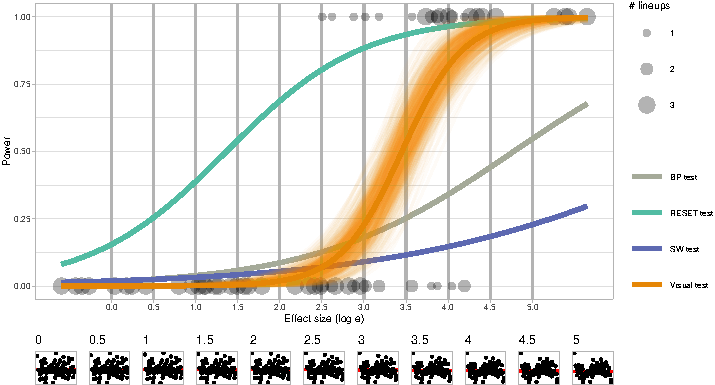
\includegraphics[width=1\linewidth]{paper_comparison_files/figure-latex/polypower-1} 

}

\caption{Comparison of power between different tests for non-linear patterns (uniform fitted values only). Main plot shows the power curves estimated using logistic regression, with dots indicating human evaluations of lineups. Surrounding lines of the visual test show the estimated power of 500 bootstrap samples. Small row of plots shows typical residual plots corresponding to specific effect sizes, marked by dashed lines in main plot. Where would you draw the line of too much non-linearity in the residuals? For the RESET test this is around log effect size 2.5, but for the visual test it is around 3.5.}\label{fig:polypower}
\end{figure}

\begin{figure}

{\centering 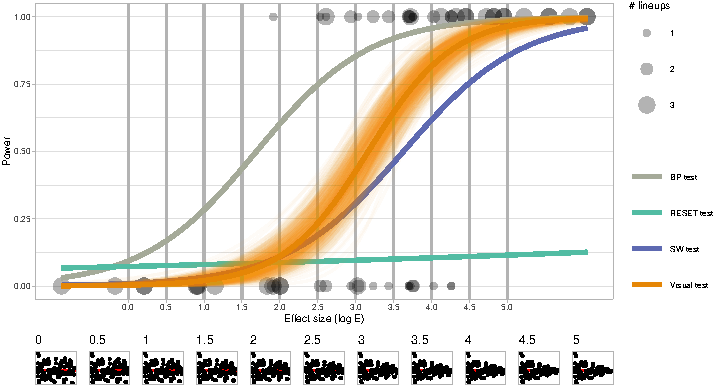
\includegraphics[width=1\linewidth]{paper_comparison_files/figure-latex/heterpower-1} 

}

\caption{Comparison of power between different tests for heteroskedasticity patterns (uniform fitted values only). Main plot shows the power curves, with dots indicating human evaluations of lineups. Surrounding lines of the visual test show the estimated power of 1000 bootstrap samples. Small row of plots shows typical residual plots corresponding to specific effect sizes, marked by dashed lines in main plot. Where would you draw the line of too much heteroskedasticity in the residuals? For the BP test this is around log effect size 2.5, but for the visual test it is around 3.5.}\label{fig:heterpower}
\end{figure}

\hypertarget{comparison-of-test-decisions-based-on-p-values}{%
\subsection{\texorpdfstring{Comparison of test decisions based on
\(p\)-values}{Comparison of test decisions based on p-values}}\label{comparison-of-test-decisions-based-on-p-values}}

\begin{figure}

{\centering 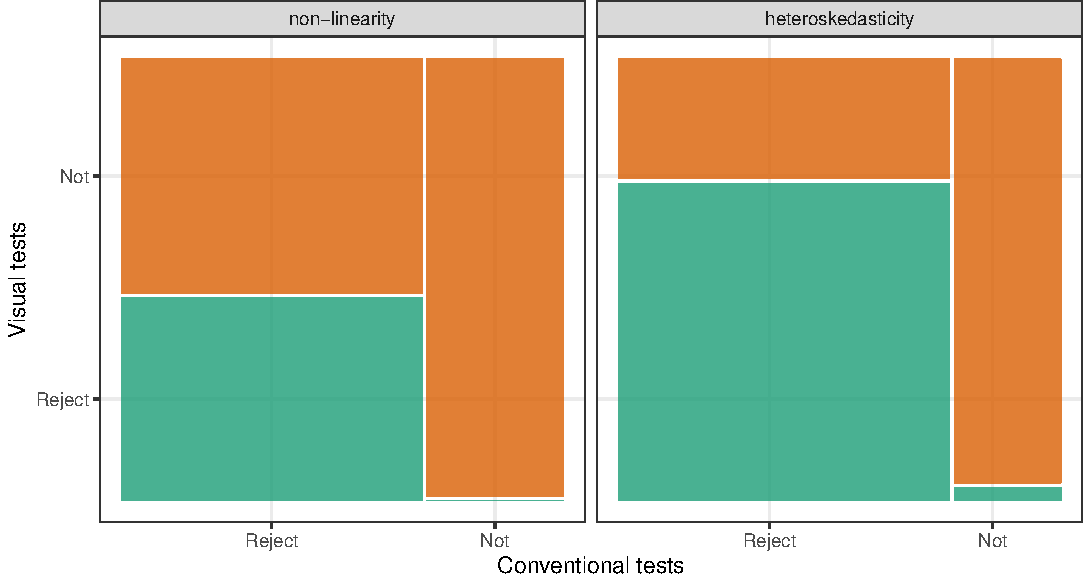
\includegraphics[width=1\linewidth]{paper_comparison_files/figure-latex/p-value-comparison-1} 

}

\caption{Rejection rate ($p$-value $\leq0.05$) of visual test conditional on the conventional test decision on non-linearity (left) and heteroskedasticity (right) lineups (uniform fitted values only) displayed using a mosaic plot. The visual test rejects less frequently than the conventional test. We would generally expect that the visual test would only reject when the conventional test does. Surprisingly, there is one lineup in the heteroskedasticity study where this is not the case. }\label{fig:p-value-comparison}
\end{figure}

The power comparison illustrates that appropriate conventional tests
will reject \(H_0\) more aggressively than visual tests. In this
section, we explore how often they agree with each other by
investigating the rejections for the two model designs based on
\(p\)-values for each lineup.

Figure \ref{fig:p-value-comparison} provides a mosaic plot showing the
rejection rate of visual tests and conventional tests for both
non-linearity patterns and heteroskedasticity patterns.

For lineups containing non-linearity patterns, conventional tests reject
69\% and visual tests reject 32\% of the time. Of the lineups rejected
by the conventional test, 46\% are rejected by the visual test, that is,
approximately half as many as the conventional test. There are no
lineups that are rejected by the visual test but not by the conventional
test.

In terms of lineups containing heteroskedasticity patterns, 76\% are
rejected by conventional tests, while 56\% are rejected by visual tests.
When the conventional test rejects a lineup, there is a great chance
(73\%) the visual test will also reject it.

Surprisingly, the visual test rejects 1 of the 33 (3\%) of lineups where
the conventional test does not reject. Figure \ref{fig:heter-example}
shows this lineup. The data plot in position seventeen displays a
relatively strong heteroskedasticity pattern, and has a strong effect
size (\(log_e E=4.02\)). This is reflected by the visual test
\(p\text{-value} = 0.026\), but the Breusch-Pagan test
\(p\text{-value} = 0.056\), slightly above the significance cutoff of
\(0.05\). This lineup was evaluated by 11 subjects, it has experimental
factors \(n=50\) (small sample size), \(\sigma=1\), and a uniform
distribution for the fitted values. It must be the small sample size
that may have resulted in the lack of detection.

\begin{figure}

{\centering 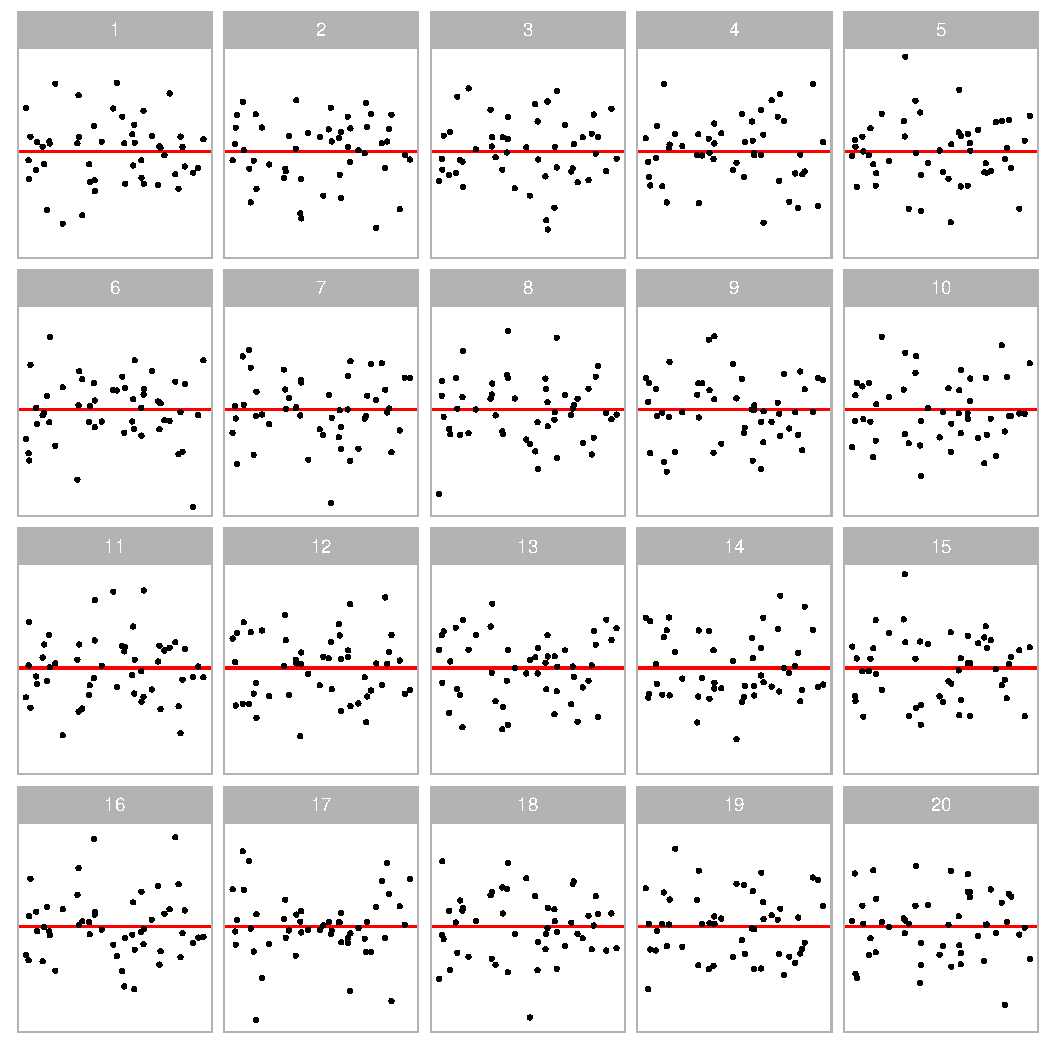
\includegraphics[width=1\linewidth]{paper_comparison_files/figure-latex/heter-example-1} 

}

\caption{The single heteroskedasticity lineup that is rejected by the visual test but not by the BP test. The data plot at panel 17 contains a "Butterfly" shape. It has effect size $ = 3.76$, somewhat surprising that it is not detected by the BP test.}\label{fig:heter-example}
\end{figure}

\hypertarget{effect-of-shape-of-non-linearity}{%
\subsection{Effect of shape of
non-linearity}\label{effect-of-shape-of-non-linearity}}

A primary factor contributes to the non-linearity model is the shape of
the non-linearity pattern. According to Figure
\ref{fig:poly-power-uniform-j}, conventional tests have roughly the same
power in testing shapes constructed from low orders of Hermite
polynomials. But the power in testing the ``Triple-U'' shape drops
significantly. To understand why this is, one needs to return to the way
the RESET test is applied. It requires a parameter indicating degree of
fitted values to test for, and the recommendation is to generically use
four (\citet{ramsey_tests_1969}). However, the ``Triple-U'' shape
constructed from the Hermite polynomials use power up to 18. If the
RESET test had been applied using a higher power no less than six, the
power curve of ``Triple-U'' shape will only slight lower than the power
curve of ``M'' shape. The recommendation of the polynomial power for the
RESET should be revised, perhaps. This illustrates the sensitivity of
conventional testing to the parameters, and it also points to a
limitation that one needs to know the data generating process in order
to set the parameters for the test.

For visual tests, based on the orders of the Hermite polynomials, we
expect the ``U'' shape will be the easiest one to be detected by
subjects followed by the ``S'', ``M'' and ``Triple-U'' shape. From
Figure \ref{fig:poly-power-uniform-j}, it can be observed that the power
curves are mostly aligned with our expectation, except for the ``M''
shape, which is the easiest shape to be detected. This implies the
visibility of the shape do not strictly follow the degree of the
polynomials.

\begin{figure}

{\centering 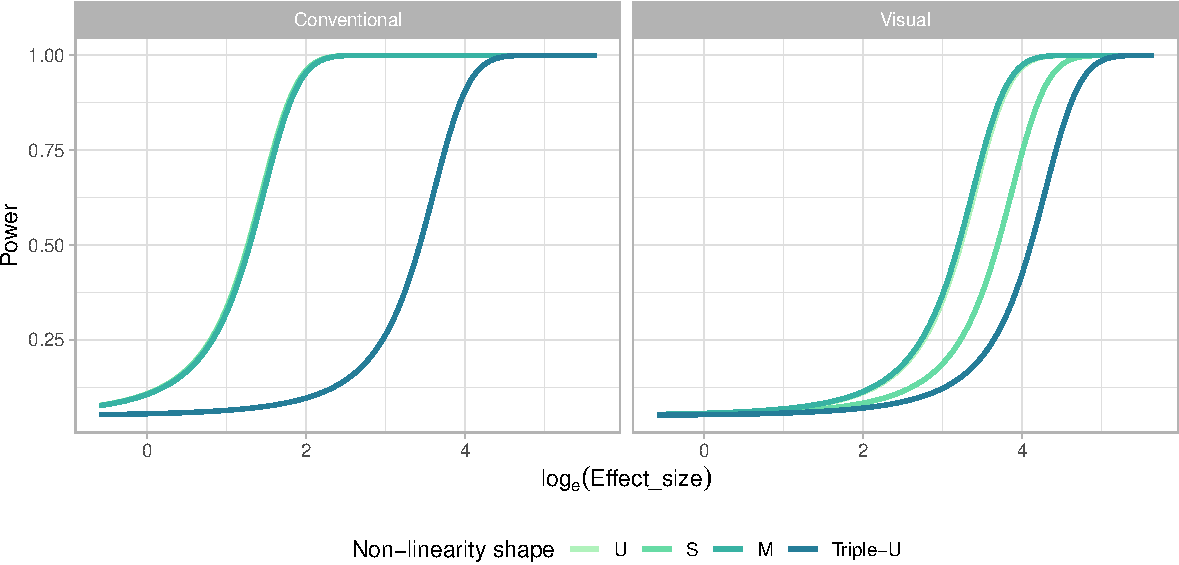
\includegraphics[width=1\linewidth]{paper_comparison_files/figure-latex/poly-power-uniform-j-1} 

}

\caption{Power of conventional tests and visual tests on lineups containing four different non-linearity shapes. Power curves with higher order of non-linearity are drawn with deeper colours. The default RESET tests under-perform significantly in detecting "Triple-U" shape. To achieve a similar power as other shapes, a higher order polynomial parameter needs to be used for the RESET test. But this means the order needs to be known prior to testing.}\label{fig:poly-power-uniform-j}
\end{figure}

\hypertarget{effect-of-shape-of-heteroskedasticity}{%
\subsection{Effect of shape of
heteroskedasticity}\label{effect-of-shape-of-heteroskedasticity}}

We have also investigated the impact of different heteroskedasticity
shapes on power of conventional tests and visual tests. In theory, the
``Left-triangle'' and the ``Right-triangle'' shapes are functionally
identical from the point of view of a Breusch-Pagan test. As shown in
Figure \ref{fig:heter-power-uniform-a}, this is indeed the case where
little difference between the power curves can be perceived. Similarly,
visual tests should have the same power in detecting these two shapes if
they are equally likely to be identified. However, it can be observed
from Figure \ref{fig:heter-power-uniform-a} that the power curve for the
``Left-triangle'' shape is higher than the one for the
``Right-triangle'' shape, indicating a potential favour of orientation
by human, which is worth to be explored in future studies. Besides, the
chance of detecting the ``Butterfly'' shape by both conventional and
visual tests are much higher than other two shapes.

\begin{figure}

{\centering 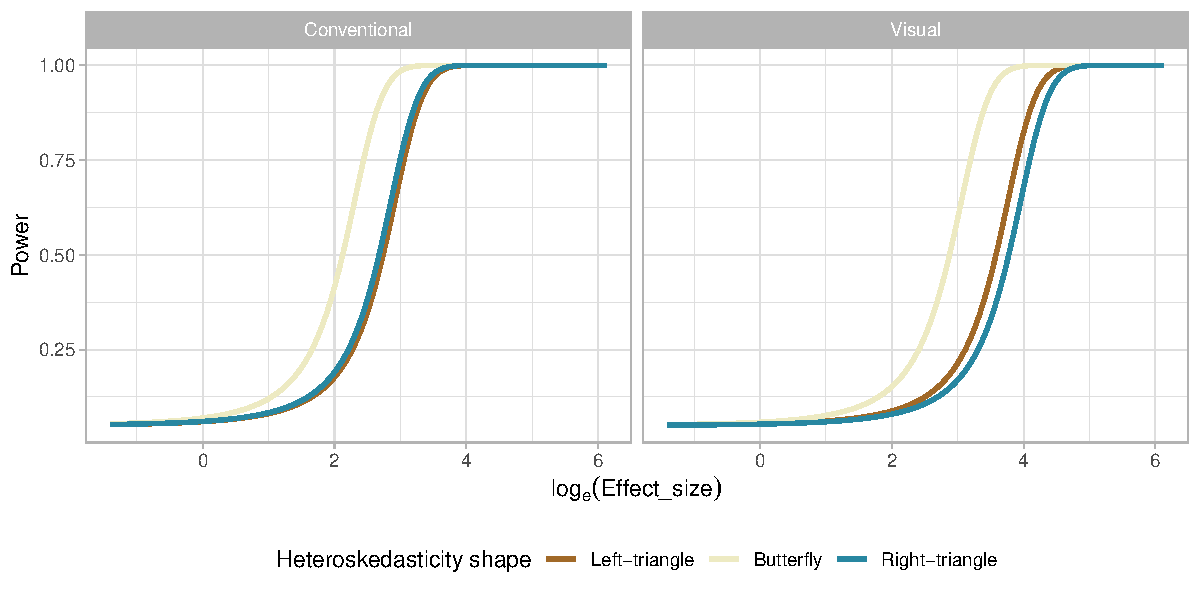
\includegraphics[width=1\linewidth]{paper_comparison_files/figure-latex/heter-power-uniform-a-1} 

}

\caption{Power of conventional tests and visual tests on lineups produced by the heteroskedasticity model with three different shapes controlled by the parameter $a$.}\label{fig:heter-power-uniform-a}
\end{figure}

\hypertarget{effect-of-fitted-value-distributions}{%
\subsection{Effect of fitted value
distributions}\label{effect-of-fitted-value-distributions}}

The prediction in a regression model is \(E(Y|X)\), that is, it is
conditional on observed values of the predictors. The distribution of
\(X\), or consequently \(\hat{Y}\), may however affect the ability to
read any patterns in the residuals. The four distributions of fitted
values, used in this experiment, were designed to examine this.

Figure \ref{fig:different-x-dist-poly-power} illustrates the change of
power of visual tests and conventional tests for different fitted
distributions used in the non-linearity model and the heteroskedasticity
model. Note that we have collected more evaluations on lineup with
uniform fitted value distribution, and the number of evaluations on a
lineup will have an impact on the power of the visual test. To have a
fair comparison, the five evaluations used in the power estimation are
randomly sampled from the total eleven evaluations for each lineup with
uniform fitted value distribution. The sampling process has been
repeated 500 times to visualize the variation.

For visual tests, the power curves for normal distribution and lognormal
distribution are lower than other two distributions, which are all even.
For non-linearity patterns, the power curve of normal distribution is
slightly greater than the one for lognormal distribution. And the margin
is even larger for heteroskedasticity patterns. This suggests skewness
can affect the degree of presence of the visual pattern.

For non-linearity patterns, we do not observe significant difference in
power of visual test between uniform distribution and discrete uniform
distribution, but the normal distribution and the lognoraml distribution
have lower power than the previous two. In terms of conventional tests,
the discrete uniform distribution is the one with the greatest power,
followed by lognormal, uniform and the normal distribution.

For heteroskedasticity patterns, the power of visual test on lineups
with uniform distribution has the greatest power. This is as expected
since other three distributions could reduce the chance of revealing the
underlying visual pattern because of uneven data points. The power of
visual test under the discrete uniform distribution has a relatively
great. Considering for heteroskedasticity, the visual patterns are
usually detected by connecting the maximum and minimum residuals
separately at different fitted values. It will not be greatly affected
by the discrete uniform distribution compared to the uniform
distribution. Again, visual tests have low power on lineups with the
normal distribution and the lognormal distribution. It indicates
skewness and unevenness can reduce the detection rate of the visual
pattern. In the case of conventional tests, the discrete uniform
distribution consistently perform well, followed by uniform, normal and
the lognormal distribution.

In regards of the type of the simulation model, the power of visual
tests under different fitted value distributions are substantially lower
than the corresponding conventional tests, which is consistent with the
result reported in the previous sections.

\begin{figure}

{\centering 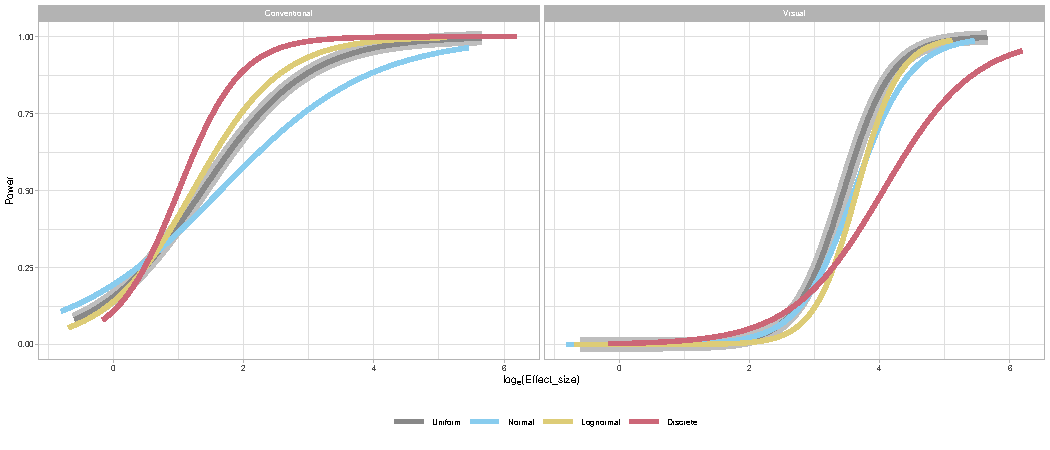
\includegraphics[width=1\linewidth]{paper_comparison_files/figure-latex/different-x-dist-poly-power-1} 

}

\caption{Comparison of power on lineups with different fitted value distributions, for conventional tests and visual tests. For visual tests, all the power curves are estimated using five evaluations on each lineup. For lineups with uniform fitted value distribution, the five evaluations are randomly sampled from the total eleven evaluations. The sampling process has been repeated for 500 times and the corresponding power curves are drawn with transparent grey lines. For both types of tests power does change. The discrete fitted value distribution substantially lowers the power of visual tests for non-linearity patterns in residual plots. For heteroskedasticity patterns, normal and lognormal distributions produce lower power for both types of tests.}\label{fig:different-x-dist-poly-power}
\end{figure}

\hypertarget{conclusion}{%
\section{Conclusion}\label{conclusion}}

Motivated by the advice of regression analysis experts, that residual
plots as opposed to conventional tests are an indispensible methods for
assessing model fit, a human subjects experiment was conducted using
visual inference. The experiment tested two primary departures from good
residuals: non-linearity and heteroskedasticity.

The experiment found that conventional residual-based statistical tests
are more sensitive to departures from assumptions for residuals than
visual tests as would be evaluated by humans. That is, conventional
tests conclude there are problems with the model fit almost twice as
often as humans would. They often reject when departures in the form of
non-linearity and heteroskedasticity are not visible to a human.

One might say that this is correct behaviour, but it can be argued that
the conventional tests are rejecting when it is not necessary. Many of
these rejections happen even when downstream analysis and results would
not be significantly affected by the small departures from a good fit.
The results from human evaluations provide a more practical solution,
which reinforces the statements from regression experts that residual
plots are an indispensible method for model diagnostics.

Now it is important to note that residual plots need to be delivered as
a lineup, where it is embedded in a field of null plots. This enables a
careful calibration for reading structure in residual plots. XXX More
here

However, human evaluation of residuals is expensive. It is
time-consuming, and laborious. This is another reason why it often
appears to be ignored. With the availability of sophisticated computer
vision algorithms today, the goal of this work is to form the basis of
providing automated residual plot reading. XXX More here

The experiment also revealed some interesting details about how residual
plots are read. For the most part, the visual test performed very
similarly to the (best) conventional test only with the power curve
shifted in the less sensitive direction. Unlike the conventional tests,
where one needs to specifically test for non-linearity or
heteroskedasticity the visual test operated effectively across the range
of departures from good residuals.

As expected, if the fitted value distribution is not uniform, there is a
loss of power in the visual test. Structure is hardest to detect if
fitted values are lognormal. Also, a surprising find was that the
direction of heteroskedasticity appears to affect the ability to
visually detect it, with wedge to the right being less detectable.

\begin{enumerate}
\def\labelenumi{\arabic{enumi}.}
\setcounter{enumi}{2}
\tightlist
\item
  how does this apply more broadly than simple regression
\end{enumerate}

recommend residual vs fitted values a. measure uncertainty b.
systemically miss some structure

\begin{enumerate}
\def\labelenumi{\arabic{enumi}.}
\setcounter{enumi}{3}
\tightlist
\item
  where does this lead? Computer vision residual plot reading
\end{enumerate}

\hypertarget{acknowledgement}{%
\section{Acknowledgement}\label{acknowledgement}}

\begin{enumerate}
\def\labelenumi{\arabic{enumi}.}
\tightlist
\item
  software tools
\item
  point to github repo (create a new one)
\item
  summarise the supplementary material
\end{enumerate}

\newpage

\begin{enumerate}
\def\labelenumi{\arabic{enumi}.}
\tightlist
\item
  put \#eval in appendix
\item
  examine batch effect in appendix
\item
  compute the power of RESET test with different orders (considering
  dof) (focus on simple pattern possibly?)
\end{enumerate}

\bibliographystyle{tfcad}
\bibliography{paper.bib}





\end{document}
